\documentclass{standalone}
\usepackage{tikz}
\usepackage{verbatim}
\usepackage{tikz}
\usetikzlibrary{shapes.geometric, calc, positioning}

\begin{document}
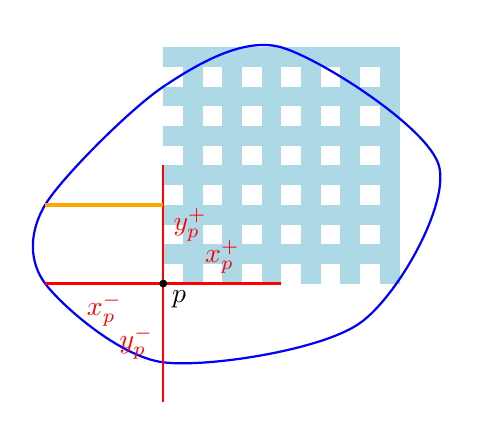
\begin{tikzpicture}

% Define the colors
\definecolor{lightblue}{RGB}{173,216,230}
\definecolor{orange}{RGB}{255,165,0}
\definecolor{red}{RGB}{255,0,0}

% Draw the background pattern
\fill[lightblue] (0,0) -- (3,0) -- (3,3) -- (0,3) -- cycle;
\foreach \x in {0,0.5,...,3}
    \foreach \y in {0,0.5,...,3}
        \fill[white] (\x,\y) rectangle +(0.25,0.25);

% Define the main shape
\draw[blue, thick] plot[smooth cycle] coordinates {(-1.5,1) (0,2.5) (1.5,3) (3.5,1.5) (2.5,-0.5) (0,-1) (-1.5,0)};

% Draw the cross lines
\draw[red, thick] (0,0) -- (1.5,0) node[midway, above] {$x_p^+$};
\draw[red, thick] (0,0) -- (-1.5,0) node[midway, below] {$x_p^-$};
\draw[red, thick] (0,0) -- (0,1.5) node[midway, right] {$y_p^+$};
\draw[red, thick] (0,0) -- (0,-1.5) node[midway, left] {$y_p^-$};

% Draw the central point
\node[circle, fill=black, inner sep=1pt] at (0,0) {};

% Draw the orange line
\draw[orange, ultra thick] (-1.5,1) -- (0,1);

% Label the central point
\node at (0.2,-0.2) {$p$};

\end{tikzpicture}
\end{document}